% main.tex

\section{Perturbative Integrability}

In this section we start attacking the problem of finding the spectrum and as expected we begin with perturbation theory.
Starting at weak coupling we quickly stumble upon an amazing feature of the theory, so-called integrability, which allows one to apply numerous techniques that greatly simplify the problem.
We demonstrate integrability from the string theoretic perspective at strong coupling as well, which suggests a unified picture of the integrable structure embedded in the theory persisting to all loops.
After discussing results achievable via perturbative integrability we finish off with our first exact result, the slope function, which in turn allows one to extract novel information about the spectrum.

\subsection{One loop at weak coupling}

We begin with two point correlation functions of local operators.
In any conformal field theory they are constrained by symmetry, namely for operators that are eigenvalues of dilatations they have the following form at all loop levels
\begin{equation}
	\left< \mathcal{O}(x) \, \tilde{\mathcal{O}}(y) \right> \approx \frac{1}{|x-y|^{2\Delta}},
\end{equation}
where $\Delta$ is the scaling dimension of the operator and we ignore unphysical normalization factors. 
Classically $\Delta = \Delta_0$ is simply the mass dimension, but at the quantum level it receives radiative corrections and acquires an anomalous dimension $\gamma$, such that $\Delta(g_{YM}) = \Delta_0 + \gamma(g_{YM})$, where the anomalous dimension depends on the coupling. 
Usually the corrections are small and the correlator can be expanded perturbatively.
Of course one has to be careful here, as expanding in $\gamma$ would result in expressions like $\log|x-y|$, which do not make sense. 
To that end we introduce a scale $\mu$ and expand the following quantity instead 
\begin{equation}
	\mu^{-2\gamma} \left< \mathcal{O}(x) \, \tilde{\mathcal{O}}(y) \right> \approx \frac{1}{|x-y|^{2\Delta_0}} \left(1 - \gamma \log \mu^2 |x-y|^2 \right),
	\label{eq:anomdim_expansion}
\end{equation}
however we will formally assume that the factor $\mu^{-\gamma}$ is absorbed into the field definition and thus we will ignore it from now on. We can now take some explicit local operator $\mathcal{O}(x)$, calculate the correlator using perturbation theory and read off the anomalous dimension $\gamma$.
Let us start with a very simple chiral primary operator 
\begin{equation}
	\Psi = \tr \, Z^L  = {Z^a}_b {Z^b}_c \dots {Z^l}_a,
	\label{eq:primary_op}
\end{equation}
where the complex scalar field $Z$ and its conjugate $\tilde{Z}$ have the standard tree level correlators
\begin{equation}
	\left< {Z^a}_b(x) {{\tilde{Z^{b'}}}}_{a'}(y) \right>_{\mathrm{tree}} \approx \frac{{\delta^a}_{a'} {\delta_b}^{b'}}{|x-y|^{2}}.
	\label{eq:z_correlator}
\end{equation}  
In order to find the anomalous dimension of the chiral primary operator $\Psi$ we must calculate $<\Psi(x) \tilde{\Psi}(x)>$. We do this by using Wick's theorem and plugging in the two-point correlator (\ref{eq:z_correlator}), which produces a lot of terms with delta function contractions between the adjoint indices. Some examples are
\begin{subequations}
	\begin{equation} 
	\dots {\delta^{a'}}_{a} \; {\delta^{a}}_{a'} \; {\delta^{b'}}_{b} \; {\delta^{b}}_{b'} \; {\delta^{c'}}_{c} \;  {\delta^{c}}_{c'} \; \dots 
	\end{equation}
	\vspace{-22pt}
	\begin{equation}
	\dots {\delta^{a'}}_{c} \; {\delta^{c}}_{a'} \; {\delta^{b'}}_{a} \; {\delta^{a}}_{b'} \; {\delta^{c'}}_{b} \;  {\delta^{b}}_{c'} \; \dots 
	\end{equation}
	\begin{equation}
	\dots {\delta^{a'}}_{a} \; {\delta^{a}}_{b'} \; {\delta^{c'}}_{b} \; {\delta^{b}}_{a'} \; {\delta^{b'}}_{c} \;  {\delta^{c}}_{c'} \; \dots 
	\end{equation}
	\label{eq:delta_contractions}
\end{subequations}
These contractions have a graphical interpretation. Consider the scalar field ${Z^a}_b$ as a dot and each contraction of the adjoint indices as a line connecting these dots, then the chiral primary operator $\Psi$ is simply a circle due to the trace. Wick's theorem says that in order to find the correlator $<\Psi(x) \tilde{\Psi}(x)>$ we must sum all possible ways we can connect the dots in the circle of $\Psi$ to the dots in the circle of $\tilde{\Psi}$. All the delta function contractions that we get after expanding the correlator represent precisely all the possible ways we can contract the dots in the circles. The three excerpts of contractions shown in (\ref{eq:delta_contractions}) can be represented graphically as shown in fig. \ref{fig:planar_nonplanar}. One can immediately notice that the first two are planar, while the third one is intersecting itself. Evaluating the three contractions we immediately see that planar ones produce a factor of $N^3$ while the non-planar one produces a factor of $N$, i.e. non-planar diagrams are suppressed and we can discard them once we take the planar limit $N \rightarrow \infty$. 
\begin{figure}[t]
\centering
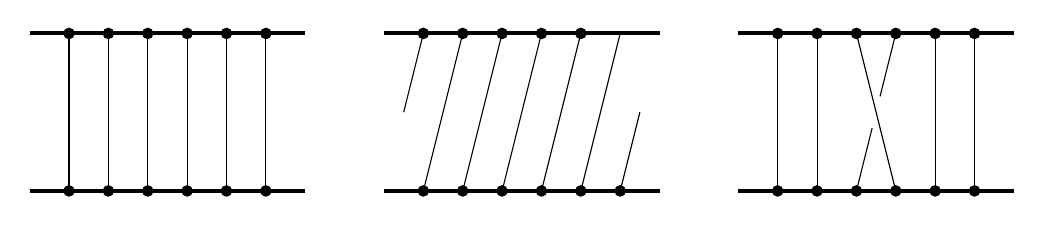
\begin{tikzpicture}[scale=0.5,every node/.style={draw,shape=circle,fill=black,scale=0.4}]
	
	%\draw[help lines] (0,0) grid (29,5);

	\def\height{4}
	\def\width{7}
	\def\gap{2}
	
	\begin{scope}[shift={(\gap,0)}]
	
		\draw[line width=0.5mm] (0,0) -- (\width,0);
		\draw[line width=0.5mm] (0,\height) -- (\width,\height);
		
		\foreach \x in {1,2,3,4,5,6} {
			\node at (\x, 0) {}; \node at (\x, \height) {};
			\draw (\x,0) -- (\x,\height);
		}

	\end{scope}
	
	\begin{scope}[shift={(\width+2*\gap,0)}]
	
		\draw[line width=0.5mm] (0,0) -- (\width,0);
		\draw[line width=0.5mm] (0,\height) -- (\width,\height);
		
		\foreach \x in {1,2,3,4,5} {
			\node at (\x, 0) {}; \node at (\x, \height) {};
			\draw (\x,0) -- (\x+1,\height);
		}
		
		\node at (6, 0) {}; ;
		
		\draw (0.5, \height / 2) -- (1,\height);
		\draw (6,0) -- (6.5,\height / 2);

	\end{scope}
	
	\begin{scope}[shift={(2*\width+3*\gap,0)}]
	
		\draw[line width=0.5mm] (0,0) -- (\width,0);
		\draw[line width=0.5mm] (0,\height) -- (\width,\height);
		
		\foreach \x in {1,2,5,6} {
			\node at (\x, 0) {}; \node at (\x, \height) {};
			\draw (\x,0) -- (\x,\height);
		}
		
		\draw (3,0) -- (3.4, 0.4 * \height); \draw (3.6, 0.6 * \height) -- (4, \height);
		\draw (4,0) -- (3,\height);
		
		\node at (3, 0) {}; \node at (3, \height) {};
		\node at (4, 0) {}; \node at (4, \height) {};

	\end{scope}
	
\end{tikzpicture}
\caption{Possible types of Wick contractions (vertical lines) between single trace operators. The constituent scalar fields are represented by dots in the horizontal lines, which represent the successive index contractions due to the trace. First two figures are examples of planar contractions while the last one is an example of a non-planar contraction.}
\label{fig:planar_nonplanar}
\end{figure}
All that's left then are cyclic permutations of lines by shifting all of them as seen in fig. \ref{fig:planar_nonplanar} while going from (a) to (b). 
There are $L-1$ shifts that can be done in this way, since after making a full circle we return to the initial configuration. 
Thus finally for the chiral primary correlator at tree level we find
\begin{equation}
	\left< \Psi(x) \, \tilde{\Psi}(y) \right>_{\mathrm{tree}} \approx \frac{L N^L}{|x-y|^{2L}},
\end{equation}
where $N^L$ comes from the contractions and $L$ from all the possible planar ways we can contract. 
This can easily be generalized for correlators of operators with arbitrary scalar fields $\Phi_{I_1 I_2 \dots I_L}(x) = \tr \left[ \Phi_{I_1}(x) \Phi_{I_2}(x) \dots \Phi_{I_L}(x) \right]$ to
\begin{equation}
	\left< \Phi_{I_1 I_2 \dots I_L}(x) \, \tilde{\Phi}^{J_1 J_2 \dots J_L}(y)  \right>_{\mathrm{tree}} \approx \frac{1}{|x-y|^{2L}} \left( \delta_{I_1}^{J_1} \delta_{I_2}^{J_2} \dots \delta_{I_L}^{J_L} + \mathrm{cycles} \right),
	\label{eq:tree_correlator}
\end{equation}
where ``cycles'' refers to terms with the $J$ indices pushed. 
$I$ and $J$ are flavor indices, the color indices are suppressed.
 
So far so good, but in order to calculate anomalous dimensions we have to go beyond tree level. 
This may seen like a highly non-trivial thing to do, since we expect not only scalar interactions, but also gluon exchanges and fermion loops appearing. 
Luckily the symmetry of the theory allows one to calculate all gluon and fermion effects in one go. 
First let's concentrate on the bosonic sector of the theory ignoring gluons. 
The action (\ref{eq:n4_action}) contains a single scalar-only interaction term
\begin{eqnarray}
S_{\Phi} & = &  \frac{g_{YM}^2}{4} \sum_{I,J} \int d^4 x \, \tr \, [\Phi_I, \Phi_J] [\Phi_I, \Phi_J] \nonumber \\
& = & - \frac{g_{YM}^2}{4} \sum_{I,J} \int d^4 x \, \left( \tr \, [\Phi_I\Phi_I\Phi_J\Phi_J] - \tr \, [\Phi_I\Phi_J\Phi_I\Phi_J]  \right).
\end{eqnarray} 
In order to calculate the correlator (\ref{eq:tree_correlator}) at one-loop level, one should insert this term and Wick contract. 
Just like in tree level, we only have to keep planar diagrams. 
For the interaction terms this means that only neighbouring fields can interact. 
This drastically reduces the number of terms we get after Wick contracting. 
Because of that it is enough to consider a length two operator $\Phi_{I_k I_{k+1}}$ and with a bit of work one can show that at one-loop level we get
\begin{eqnarray}
	 & \left< \Phi_{I_k I_{k+1}}(x) \, \tilde{\Phi}^{J_k J_{k+1}} \right>_{\mathrm{one-loop}}  = \frac{\lambda}{16\pi^2} \frac{\log (\mu^2|x-y|^2)}{|x-y|^{2L}} \times \nonumber \\ 
	& \times  \left( 2 {\delta_{I_k}}^{J_{k+1}} {\delta_{I_{k+1}}}^{J_{k}} - \delta_{I_k I_{k+1}} \delta^{J_k J_{k+1}} - {\delta_{I_k}}^{J_{k}} {\delta_{I_{k+1}}}^{J_{k+1}} \right),
	\label{eq:loop_correlator}
\end{eqnarray}
where $\lambda = g_{YM}^2 N$ is the t'Hooft coupling. 
Comparing this to (\ref{eq:tree_correlator}) we see that effectively the interactions permute and contract the delta function indices. 
We can introduce exchange and trace operators to make this explicit. 
The permutation operator, also called the exchange operator, $\mathcal{P}_{l,l+1}$ is defined by it's action on a set of delta functions as
\begin{equation}
	\mathcal{P}_{l,l+1} \; {\delta_{I_{1}}}^{J_{1}} \dots {\delta_{I_{l}}}^{J_{l}} {\delta_{I_{l+1}}}^{J_{l+1}} \dots {\delta_{I_{L}}}^{J_{L}} = {\delta_{I_{1}}}^{J_{1}} \dots {\delta_{I_{l}}}^{J_{l+1}} {\delta_{I_{l+1}}}^{J_{l}} \dots {\delta_{I_{L}}}^{J_{L}}
\end{equation}
and the trace operator $\mathcal{K}_{l,l+1}$ is defined as
\begin{equation}
	\mathcal{K}_{l,l+1} \; {\delta_{I_{1}}}^{J_{1}} \dots {\delta_{I_{l}}}^{J_{l}} {\delta_{I_{l+1}}}^{J_{l+1}} \dots {\delta_{I_{L}}}^{J_{L}} = {\delta_{I_{1}}}^{J_{1}} \dots {\delta_{I_l I_{l+1}}} {\delta}^{J_{l} J_{l+1}} \dots {\delta_{I_{L}}}^{J_{L}}.
\end{equation}
Using these operators we can rewrite the correlator in (\ref{eq:loop_correlator}) in a more compact notation
\begin{eqnarray}
	  \left< \Phi_{I_k I_{k+1}}(x) \, \tilde{\Phi}^{J_k J_{k+1}} \right>_{\mathrm{one-loop}} = &  \nonumber \\
	  = \frac{\lambda}{16\pi^2} \frac{\log (\mu^2|x-y|^2)}{|x-y|^{2L}} 
	 & \left( 2 \; \mathcal{P}_{k,k+1} - \mathcal{K}_{k,k+1} - 1 \right) \delta_{I_k}^{J_{k}} \delta_{I_{k+1}}^{J_{k+1}}.
\end{eqnarray}
This result includes four scalar interactions only, however as mentioned before at one-loop level we can also have gluon interactions and fermion loops in scalar propagators. 
The nice thing about these is that such interactions don't alter the flavor index structure, i.e. there are no permutations or traces. 
Basically this happens because the gluon transforms trivially under R-symmetry and hence can't change the flavor index (which transforms under R-symmetry). 
Similarly, fermions can only appear in loops altering scalar self-energies, hence they also leave the flavor structure intact.
Thus all of these interactions contribute a constant term $C$, which we can determine later. We can generalize our one-loop result with all interactions included for operators of arbitrary length,
\begin{equation}
\begin{split}
	 & \left< \Phi_{I_1 I_2 \dots I_L}(x) \, \tilde{\Phi}^{J_1 J_2 \dots J_L}(y)  \right>_{\mathrm{one-loop}}
	  = \frac{\lambda}{16\pi^2} \frac{\log (\mu^2|x-y|^2)}{|x-y|^{2L}} \times \nonumber \\
	 & \times \sum_{l=1}^L \left( 2 \; \mathcal{P}_{l,l+1} - \mathcal{K}_{l,l+1} - 1 + C\right)
	  \left( \delta_{I_1}^{J_1} \delta_{I_2}^{J_2} \dots \delta_{I_L}^{J_L} + \mathrm{cycles} \right).
\end{split}
\end{equation}
Combining this with the tree level result (\ref{eq:tree_correlator}) and comparing to the general expression of a two-point function at one-loop level (\ref{eq:anomdim_expansion}) we can deduce the anomalous dimension $\gamma$, which now becomes an operator $\Gamma$ because of the flavor mixing. 
It is given by
\begin{equation}
	\Gamma = \frac{\lambda}{16\pi^2}\sum_{l=1}^L \left( - 2 \; \mathcal{P}_{l,l+1} + \mathcal{K}_{l,l+1} + 1 - C\right).
\end{equation}
At first sight it may seem strange that what was supposed to be a number, i.e. a correction to the mass dimension of an operator has turned out to be an operator acting on the flavor space, i.e. a matrix. 
But this is very natural and in fact expected, since interactions can change the flavor of fields and we can't be sure that an operator at the quantum level has the same flavor indices as it does at the classical level. 
This line of thinking may lead to a natural question, why do we have mixing between the scalars only and not between all the fields in the theory including fermions, which miraculously do not appear. 
It turns out that this is a one-loop feature only and mixing becomes a problem at higher loop levels \cite{Minahan:2002ve}. 

Now that we have acknowledged that the anomalous dimension is a matrix and found an expression for it, the next logical step would be diagonalizing it and finding the flavor eigenstates. 
One example of such an eigenstate is the chiral primary operator $\Psi$. 
Since it contains scalar fields of only one type, the permutation and trace operators act trivially on it. Thus we see that
\begin{equation}
	\Gamma \, \Psi = \frac{\lambda}{16\pi^2}\sum_{l=1}^L \left( -2 + 1 - C \right) \Psi,
\end{equation}
but we already saw that a chiral primary has an anomalous dimension of zero, which then fixes the constant $C$ to $-1$. 
And finally we get
\begin{equation}
	\Gamma = \frac{\lambda}{16\pi^2}\sum_{l=1}^L \left(2 - 2 \; \mathcal{P}_{l,l+1} + \mathcal{K}_{l,l+1} \right).
\end{equation}
A keen eye might already notice that this expression resembles a Hamiltonian of a spin chain. 
In fact, this is hardly surprising, since from the very beginning we were talking about fields as points in some closed line, which indeed resembles a spin chain. 
Furthermore the correlators that we were calculating are nothing more that propagators from one state of the chain to another, hence no wonder that the operator describing this evolution looks like a Hamiltonian for a spin chain. 
This identification is very useful, because the spin chains that appear in AdS/CFT are integrable and can be solved exactly, which gives us hope that we can apply the same techniques here and solve the spectral problem in $\N=4$ exactly. 
The first steps towards this goal were outlined in the seminal paper \cite{Minahan:2002ve}, which launched the integrability program in AdS/CFT. 
However saying that the spectral problem can be solved exactly in this particular case is too strong, since we are only at one-loop level. 
Nevertheless one can apply the same techniques going beyond one-loop level, as we shall soon see in the coming sections. 


\subsubsection{The $\mathfrak{su}(2)$ sector}

In the previous section we considered single trace operators potentially containing all six scalar fields, we also mentioned that at higher loops the remaining fields of the theory start mixing in, i.e. the scalar sector is only closed at one-loop level.
However it is easy to see that there exist sectors that are closed at all loops.
From the algebra of the theory we know that dilatations commute with Lorentz and R-symmetries at any value of the coupling, hence it must follow that all the coefficients in
\beq
	D = \sum_n \lambda^n D^{(2n)},
\eeq
where in particular $D^{(2)} \equiv \Gamma$, commute with  Lorentz and R-symmetry generators. 
Thus we conclude that only operators with the same bare dimensions, Lorentz charges and R-charges can mix when acting with the anomalous dimension matrix.

Arguably the simplest possible closed sector is the so-called $\mathfrak{su}(2)$ sector, containing only two scalar fields $X$ and $Z$. 
An operator with $M$ and $L-M$ scalars $X$ and $Z$ has the charges $(0, 0; L; M, L-M, 0)$, the only other operators with these charges are permutations of this operator, hence the sector is closed. 
The anomalous dimension operator in this sector is given by
\begin{equation}
	\Gamma = \frac{\lambda}{8\pi^2}\sum_{l=1}^L \left(1 - \; \mathcal{P}_{l,l+1} \right).
\end{equation}
Up to a constant factor this is the same as the Hamiltonian for the Heisenberg spin chain (also called the XXX spin chain), which is a quantum description of a one dimensional magnet. 
The Hamiltonian is given by
\begin{equation}
	\mathbf{H} = \sum_{l=1}^L \left(1 - \mathcal{P}_{l,l+1} \right),
\end{equation}
which can also be rewritten in terms of Pauli matrices as
\begin{equation}
	\mathbf{H} = 2 \sum_{l=1}^L \left( \frac{1}{4} - \vec{S}_l \cdot \vec{S}_{l+1} \right), \;\;\;\; \vec{S}_l = \frac{1}{2} \vec{\sigma}_l.
\end{equation}
Hence solving the spectral problem in $\N=4$ SYM translates into solving the Schr\"{o}dinger equation
\begin{equation}
	\mathbf{H} \, \ket{\psi} = E \, \ket{\psi},
	\label{eq:Schrodinger}
\end{equation}
where we now seek to find the energy eigenvalues for the Hamiltonian of the spin chain. 
If the chain is short, this is a trivial diagonalization problem that can be easily solved by a present day computer. 
However this problem was first solved analytically by Hans Bethe in a time when computers were still in their infancy. 
The original solution now goes by the name of \emph{coordinate Bethe ansatz} and it is by far one of the most important and beautiful solutions in physics in the past century, which is still very widely used even to this day. 
The idea is to make an educated guess for the wave function $\ket{\psi}$, plug it in to the Schr\"{o}dinger equation and determine when does it actually hold. 
This produces a set of algebraic Bethe ansatz equations for a set of variables unimaginatively called the Bethe roots. 
All observables can then be expressed in terms of these numbers as simple algebraic functions, thus transforming a diagonalization problem to an algebraic problem. 
This has an enormous advantage, since in the asymptotic limit, when the spin chain is very large, instead of diagonalizing an infinite matrix, the set of algebraic equations actually simplify and produce integral equations, which can be solved.

In the spin chain language the scalar fields can be treated as up and down spin states, i.e.
\begin{equation}
	\ket{\uparrow\,} = Z = \left( \begin{matrix} 1 \\ 0 \end{matrix} \right), \,\,\,\, \ket{\downarrow\,} = X = \left( \begin{matrix} 0 \\ 1 \end{matrix} \right),
\end{equation}
thus local single trace operators can be treated as states of a spin chain, e.g.
\begin{equation}
	\tr \left( XXZXXZX \right) = \ket{\downarrow \, \downarrow \, \uparrow \, \downarrow \, \downarrow \, \uparrow \, \downarrow \,}.
\end{equation}
Due to the cyclicity of the trace all rotations of the chain are equivalent. 
We should also specify the periodicity boundary condition
\begin{equation}
	\vec{S}_{L+1} = \vec{S}_1.
\end{equation}
The operators $\vec{S}_l$ act as Pauli matrices on the $l$'th spin site and trivially on all the others. 
Since a spin ``chain'' with a single site would have a state space $\mathbb{C}^2$, a spin chain of length $L$ has a state space $\mathbb{C}^{\otimes_L 2}$, which has $2^L$ basis vectors and the Hamiltonian is then a $2^L \times 2^L$ matrix, which we need to diagonalize. 
Working directly with Pauli matrices one can find some simple results directly, e.g. it is trivial to show that the chiral primary operator
\begin{equation}
	\ket{\Psi} = \tr \; Z^L = \ket{\uparrow \, \uparrow \, \dots \, \uparrow \,}
\end{equation}
is an eigenstate of the Hamiltonian with zero energy, i.e. it is the ferromagnetic ground state of the spin chain, which we will denote as $\ket{0}$ from now on. 
This is expected, since we know that chiral primaries have zero anomalous dimensions. 
Another eigenstate of the Hamiltonian is the \emph{single magnon} state, defined as
\begin{equation}
	\ket{p} = \sum_{n=1}^L e^{ipn} \ket{n},
\end{equation} 
where $\ket{n}$ is the ground state with the $n$'th spin flipped,
\begin{equation}
	\ket{n} = S^-_n \, \ket{0} = \ket{\uparrow \, \uparrow \, \uparrow \, \dots \, \downarrow \, \dots \, \uparrow \, \uparrow \, \uparrow \,},
\end{equation}
here $p$ is formally just a parameter, but it can be interpreted as the momentum of the excitation travelling in the spin chain. 
Due to the cyclicity of the chain the momentum is quantized,
\begin{equation}
	p = \frac{2\pi}{L} n, \,\,\,\,\, n \in \mathbb{Z},
\end{equation}
where $n$ is the mode number. 
The energy of the excitation is given by the dispersion relation
\begin{equation}
	E(p) = 4 \, \mathrm{sin}^2 \, \frac{p}{2}.
	\label{eq:magnon_energy}
\end{equation}
Now consider a two magnon state
\begin{equation}
	\ket{\psi} = \sum_{n<m} \psi(n, m) \, \ket{n,m},  \,\,\,\,\, \ket{n,m} = S^-_n \, S^-_m \, \ket{0}.
\end{equation}
The situation is not so trivial this time, since the two magnons might scatter among themselves. We now plug this into (\ref{eq:Schrodinger}) and find the conditions for $\psi(n,m)$, which are
\begin{equation}
\begin{split}
	E \, \psi(n,m) = 4 \, \psi(n,m) & -  \psi(n+1,m)  -  \psi(n-1,m) \\ 
	                              & -  \psi(n, m+1)  -  \psi(n, m-1)
\end{split}
\end{equation}
when $m > n+1$ and
\begin{equation}
	E \, \psi(n, n+1) = 2 \, \psi(n, n+1) - \psi(n-1, n+1) - \psi(n, n+2)
\end{equation}
when $m = n+1$, i.e. when the two magnons scatter. 
The solution is now a superposition of single magnon states
\begin{equation}
	\psi(n,m) = e^{ikn + ipm} + S(k,p) e^{ipn + ikm},
\end{equation}
where
\begin{equation}
	S(p,k) = \frac{\frac{1}{2} \mathrm{cot} \frac{k}{2} - \frac{1}{2} \mathrm{cot} \frac{p}{2} - i}{\frac{1}{2} \mathrm{cot} \frac{k}{2} - \frac{1}{2} \mathrm{cot} \frac{p}{2} + i}
\end{equation}
is the scattering matrix. 
As required, such a state is an eigenstate and the energy is given by
\begin{equation}
	E = E(p) + E(k),
\end{equation}
i.e. it is simply the sum of the single magnon energies. 
Finally the spin chain periodicity condition imposes the following equations
\begin{equation}
	e^{ikL} \, S(p,k) = e^{ipL} \, S(k, p) = 1.
\end{equation}
It is now straightforward to generalize this procedure, which is exactly what Bethe did. 
The wave function for $M$ spins down can be written as
\begin{equation}
	\ket{\psi} = \sum_{1 \leq l_1 < l_2 < \dots < l_M \leq L} \psi(l_1, l_2, \dots, l_M) \, S^-_{l_1} \, S^-_{l_2} \, \dots \, S^-_{l_M} \, \ket{0}.
\end{equation}
The sum is chosen in a way so as not to over count states. The Bethe ansatz is the educated guess of the wave function
\begin{equation}
	\psi(l_1, l_2, \dots, l_M) = \sum_{\sigma \, \in \; perm(1,2,\dots\,M)} A(p) \, e^{ip_{\sigma_1} l_1 + ip_{\sigma_2} l_2 + \dots + ip_{\sigma_M} l_M}, 
\end{equation}
where the sum runs over all permutations of the down spin labels $1, 2, \dots, M$. 
$p_i$ are the momenta of the down spins, which can be treated as excitations moving in the vacuum state of the spin chain. 
The ansatz then looks like a superposition of plane waves. 
As in the two magnon case, one should now plug in the ansatz and find the conditions that make it work. 
The result is a set of algebraic equations, called the \emph{Bethe equations}
\begin{equation}
	e^{ip_k L} = - \prod_{\substack{j=1 \\ j \neq k}}^M \frac{e^{ip_j} - e^{ip_k} + 1}{e^{ip_k} - e^{ip_j} + 1} \,\,\,\, \mathrm{for} \,\, k = 1,2, \dots, M
	\label{eq:bethe_coordinate}
\end{equation}
and the amplitude is given by
\begin{equation}
	A(r) = \mathrm{sign}(\sigma) \prod_{j<k} \left( e^{ip_j} - e^{ip_k} + 1 \right).
\end{equation}
These equations can be interpreted physically once rewritten as
\begin{equation}
	e^{ip_k L} \prod_{\substack{j=1 \\ j \neq k}}^M S(p_j, p_k) = 1, \,\,\,\, \mathrm{where} \,\, S(p_j, p_k) = -\frac{e^{ip_k} - e^{ip_j} + 1}{e^{ip_j} - e^{ip_k} + 1}.
	\label{eq:CBA}
\end{equation}
This is simply saying that if we take a magnon, carry it around the spin chain, the total phase change which is a result of free propagation (represented by $e^{ip_k L}$) and scattering with other magnons (due to $S(p_j,p_k)$) must be trivial.  
Changing variables to
\begin{equation}
	e^{ip_k} = \frac{u_k + i/2}{u_k - i/2}, \;\;\;\; u_k = \frac{1}{2} \, \mathrm{cot} \, \frac{p_k}{2},
\end{equation}
brings the Bethe equations (\ref{eq:bethe_coordinate}) to a more familiar form
\begin{equation}
	\left( \frac{u_k + i/2}{u_k - i/2} \right)^L = \prod_{\substack{j=1 \\ j \neq k}}^M \frac{u_k - u_j + i}{u_k - u_j - i},
\end{equation}
where now one solves for the Bethe roots $u_k$, also known as magnon rapidities. 
It is now straightforward to see that this general solution reproduces the two magnon scenario we discussed earlier. 
The energy of the $M$ magnon state is given by
\begin{equation}
	E = \sum_{k=1}^M \frac{1}{u_k^2 + 1/4},
\end{equation}
 which also agrees with the single and two magnon examples. 
 
They key thing worth noting in (\ref{eq:CBA}) is that the spin chain can be fully described in terms of the scattering matrix for just two particles, i.e. the full $M$ particle scattering matrix factorizes.
This is the defining property of integrability, since factorized scattering means that individual momenta are conserved in each two particle scattering producing a tower of conserved quantities -- just the thing one would want in an integrable system. 
 
\subsubsection{$\mathfrak{sl}(2)$ and other sectors}

sl2

\subsection{Higher loops}


The next step in solving the spectral problem is increasing the loop level. For the $\mathfrak{su}(2)$ sector this has first been done for two-loops using mainly diagrammatic methods and by fixing the structure of the operator by symmetry. The resulting dilatation operator is given by \cite{su2_loops}
\begin{equation}
	\Gamma_{2-loop} = \frac{\lambda}{8\pi^2}\sum_{l=1}^L \left(-4 + 6 \, \mathcal{P}_{l,l+1} - \left( \mathcal{P}_{l,l+1} \, \mathcal{P}_{l+1,l+2} + \mathcal{P}_{l+1,l+2} \, \mathcal{P}_{l,l+1} \right) \right).
\end{equation}
In the spin chain picture this corresponds to a Hamiltonian for a long range spin chain with two nearest neighbour interactions. This spin chain has been shown to be integrable \cite{su2_loops}. This result has been extended to three, four and five loops \cite{beisert_all_loops}. The explicit expressions for the dilatation operator at higher loops get more and more lengthy and complicated, but a pattern emerges that at loop level $l$ the dilatation operator can be identified with a Hamiltonian of a long range spin chain where at most $l$ nearest neighbours in the chain interact. What is even more remarkable is that these spin chains also turn out to be integrable \cite{three_loops}, which hints that integrability may be an all loop phenomenon. This was in part verified by solving the spectral problem in the asymptotic limit, i.e. when the spin chain length $L$ becomes infinite, but the number of excitations $M$ is kept finite. The solution is given by conjecturing a set of \emph{asymptotic Bethe ansatz equations}, which since their original inception have been extensively verified \cite{aba_tests,aba_tests2}. The equations have the same form as in the one-loop case (\ref{eq:CBA}), but the scattering function for two magnons gets modified to \cite{dorey}
\begin{equation}
	S(p_i, p_j) = \frac{u(p_i) - u(p_j) + i}{u(p_i) - u(p_j) - i} \times S_D(p_i, p_j),
\end{equation}
where $S_D(p_i, p_j)$ is the so called dressing factor (an explicit expression for it can be found in \cite{dressing}) and the rapidities are now defined as
\begin{equation}
	u(p) = \frac{1}{2} \, \mathrm{cot} \, \frac{p}{2} \, \sqrt{1 + \frac{\lambda}{\pi^2} \, \mathrm{sin}^2 \, \frac{p}{2}}.
\end{equation}
The outcome is that all one-loop results get slightly modified, e.g. the magnon dispersion relation (\ref{eq:magnon_energy}) becomes
\begin{equation}
	E(p) = \frac{8\pi^2}{\lambda} \left( \sqrt{1 + \frac{\lambda}{\pi^2} \, \mathrm{sin}^2 \, \frac{p}{2}} - 1 \right),
	\label{eq:ABA_e}
\end{equation}  
which in the low coupling limit $\lambda \rightarrow 0$ agrees with the one-loop result as it should. For many magnon states the energy is still given by the sum of individual magnon energies. It is truly remarkable that such a simple solution exists even though the Hamiltonian of the all-loop spin chain is not known. But even though such an easy generalization to an all-loop solution looks promising, it is only the first step towards the full solution of the spectral problem in $\N=4$ SYM. 

Short example of a two loop Hamiltonian, perturbative corrections for the states found above with contact terms.

\subsection{Asymptotic solution}

\beq
	\label{eq:sl2_aba}
	\( \frac{x_k^+}{x_k^-} \)^J = \prod_{j \neq k}^S \frac{x_k^- - x_j^+}{x_k^+ - x_j^-} \, \frac{1 - 1/(x_k^+ x_j^-)}{1 - 1/(x_k^- x_j^+)} \; \sigma^2(u_k, u_j), \;\;\; k = 1, \dots S
\eeq
where 
\beq
	\Delta = J + S + \gamma(g), \;\;\; \gamma(g) = \frac{i \sqrt{\lambda}}{2\pi} \sum_{j=1}^S \( \frac{1}{x_j^+} - \frac{1}{x_j^-} \)
\eeq
with
\beq
\label{eq:u_of_x}
u(x) = g \(x + \frac{1}{x}\)
\eeq

\subsubsection{A glimpse ahead: the slope function}

The asymptotic Bethe ansatz \eq{eq:sl2_aba} is the first non-trivial exact result we encountered so far, even if only valid in the asymptotic limit. In this short paragraph we will demonstrate how it can be used to find the exact \emph{slope function} $\gamma^{(1)}(g)$, which is defined as the linear term in the small $S$ expansion of the anomalous dimension, namely
\beq
	\gamma(g) = \gamma^{(1)}(g) \; S + \gamma^{(2)}(g) \; S^2 + \ord{S^3}.
\eeq
The subleading coefficient $\gamma^{(2)}(g)$ is called the \emph{curvature function} and it will be the main study object of section ??, where we also address the question of what it actually means to send an integer quantity $S$ to zero. 

The slope function was initially conjectured in \cite{Basso:2011rs} and later independently proved in \cite{Gromov:2012eg} and \cite{Basso:2012ex}, our derivation will follow the former reference. The starting point is the logarithm of the asymptotic Bethe ansatz \eq{eq:sl2_aba}, given by
\beq
	\label{eq:log_sl2_aba}
	\frac{J}{i} \log \( \frac{x_k^+}{x_k^-} \) - \sum_{j \neq k}^S \frac{1}{i} \log \( \frac{x_k^- - x_j^+}{x_k^+ - x_j^-} \, \frac{1 - 1/(x_k^+ x_j^-)}{1 - 1/(x_k^- x_j^+)} \; \sigma^2(u_k, u_j) \) = 2 \pi n_k,
\eeq
where $n_k$ is the mode number of the $k$'th Bethe root. In the small $S$ limit the number of Bethe roots also tends to zero and in this regime they stop interacting \cite{Basso:2011rs}, thus we will consider the case when $n_k = n$ and the general result will simply be a linear combination of terms with different values of $n_k$. The key idea of the derivation is assuming that the result only depends on the combination $\Lambda \equiv n \sqrt{\lambda}$ and taking the small $n$ limit. Obviously this limit is also the strong coupling limit, as $\lambda \sim 1/n^2 \rightarrow \infty$. This considerably simplifies the derivation, for starters we only need the strong coupling expansion of the dressing phase, which is given by [??]
\beq
	\log \, \sigma(u_k, u_j) \simeq -\log \( \frac{1-1/(x_k^+ x_j^-)}{1-1/(x_k^- x_j^+)} \) + i\,(u_j - u_k) \log \( \frac{x_j^- x_k^- - 1}{x_j^- x_k^+ - 1} \frac{x_j^+ x_k^+ - 1}{x_j^+ x_k^- - 1} \).
\eeq
Also, since $u_k \sim 1/n$ we can simplify the shifts in the rapidities $u_k$, namely
\beq
	x_k^\pm = x\(u_k \pm \frac{i}{2}\) = x\( \frac{1}{g} \(x_k + \frac{1}{x_k}\) \pm \frac{i}{2} \) = x_k \pm \frac{i}{2g}\frac{x_k^2}{x_k^2 - 1} + \ord{\frac{1}{g^2}}.
\eeq
Plugging in the leading order dressing phase expansion and getting rid of the shifts in the rapidities reduces the asymptotic Bethe ansatz equations \eq{eq:log_sl2_aba} to
\beq
	\sum_{j \neq k} \frac{2}{x_k - x_j} + \frac{1}{x_k} \( J + \gamma + \frac{2}{1-x_k^2} \) = \frac{\Lambda (x_k^2 - 1)}{2x_k^2}
\eeq

\beq
	\gamma = G(1) - G(-1)
\eeq

\beq
	G^2(x) + G'(x) + \( \frac{J + \gamma + 2}{x} - \frac{2x}{x^2-1} + \frac{\Lambda}{2} \frac{1-x^2}{x^2} \) G(x) = F(x)
\eeq

\beq
	F(x) = \frac{\Lambda}{2}\frac{G(0)+G'(0)x}{x^2} + \( J + \gamma + 2 \)\frac{G(0)}{x} - \frac{G(1)}{x-1} - \frac{G(-1)}{x+1}
\eeq

\beq
	\Lambda G'(0) = 2G(1) + 2G(-1) - 2G(0)(J + \gamma + 2) - \Lambda S
\eeq

\beq
	F(x) = \frac{\Lambda}{2}\( \frac{G(0)}{x^2} - \frac{S}{x} \) + \frac{G(-1)}{x(x+1)} - \frac{G(1)}{x(x-1)}
\eeq

\beq
	G(x) = \frac{x^2-1}{x^{J+2}} e^{\Lambda \frac{x^2+1}{2x}} \int_{x_0}^x dy \; F(y) \frac{y^{J+2}}{y^2-1} e^{-\Lambda \frac{y^2+1}{2y}}
\eeq

\begin{subequations}
  \begin{align}
	\Lambda(G(0)-S) - G(+1)(2J+1)+G(-1) &= 0 \\
	\Lambda(G(0)+S) + G(-1)(2J+1)-G(+1) &= 0
  \end{align}
\end{subequations}

\beq
G(x) = -\frac{\Lambda}{2}\frac{S}{J}-\frac{\gamma}{2x}-\frac{\Lambda}{4J} \frac{x^2-1}{x^{J+2}} e^{\Lambda \frac{x^2+1}{2x}} \int_0^x dy \( \gamma J y^{J-1} + \Lambda S y^J \) e^{-\Lambda \frac{y^2+1}{2y}}
\eeq

\beq
	I_\nu(\Lambda) = \frac{(-1)^{-\nu}}{2\pi i} \oint dy \; y^{\nu-1} e^{\Lambda \frac{y^2+1}{2y}}
\eeq

\beq
	\gamma J (-1)^J I_J(\Lambda) + \Lambda S (-1)^{J+1} I_{J+1}(\Lambda) = 0
\eeq

\beq
	\gamma^{(1)}(\Lambda) = \frac{\Lambda}{J} \frac{I_{J+1}(\Lambda)}{I_J(\Lambda)}
\eeq

\subsection{Strong coupling and the algebraic curve}



In the previous section we defined strings on $AdS_5 \times S^5$ in terms of the algebra current $J$, given in (\ref{eq:j_current}). This current has the property of being flat,
\begin{equation}
	dJ - J \wedge J = 0,
\end{equation}
and what is more, one can even define a one parameter family of connections from it by \cite{sakura}
\begin{equation}
\begin{split}
	L(x) = J^{(0)} & + \,\,\, \frac{x^2 + 1}{x^2 - 1} \; J^{(2)}  - \,\,\,\, \frac{2x}{x^2 - 1} \; \left( * J^{(0)} - \Lambda \right) \\ 
	 & + \sqrt{\frac{x+1}{x-1}} \; J^{(1)} + \sqrt{\frac{x-1}{x+1}} \; J^{(3)},
\end{split}
\end{equation} 
which are flat for all $x$,
\begin{equation}
	dL(x) - L(x) \wedge L(x) = 0.
\end{equation}
Here $L(x)$ is the \emph{Lax connection} and $x$ is the spectral parameter. The existence of such a set of connections signals that the theory is at least classically integrable. This can be shown by constructing the monodromy matrix
\begin{equation}
	\Omega(x) = \mathcal{P} \; \mathrm{exp} \oint_\gamma L(x),
\end{equation}
where $\gamma$ is any path wrapping the worldsheet cylinder. Since the connection is flat, by definition it is path independent and we can evaluate the integral along any $\tau = const$ loop. Furthermore, shifting the $\tau$ value corresponds to doing a similarity transformation on the monodromy matrix \cite{gromov_quasiclassical}, meaning that the eigenvalues must be time independent. Thus we have an infinite tower of conserved charges, hinting that the theory may be integrable. Denote the eigenvalues of the monodromy matrix as
\begin{equation}
	\{ e^{i\hat{p}_1(x)}, \; e^{i\hat{p}_2(x)}, \; e^{i\hat{p}_3(x)}, \; e^{i\hat{p}_4(x)} \; | \; e^{i\tilde{p}_1(x)}, \; e^{i\tilde{p}_2(x)}, \; e^{i\tilde{p}_3(x)}, \; e^{i\tilde{p}_4(x)} \}.
\end{equation} 
Here the quantities $p(x)$ are called \emph{quasi-momenta}. The bar as always denotes the $\mathbb{Z}_2$ grading and we use the convention that hatted quantities correspond to $AdS_5$ variables and quantities with tildes correspond to $S^5$. From elementary algebraic geometry we know that the zeroes of any polynomial define an algebraic curve and since the eigenvalues $e^{ip(x)}$ are the zeroes of the characteristic polynomial of the monodromy matrix, they must also define an algebraic curve. A key idea in the development of integrability was the realization that this algebraic curve also known as the \emph{spectral curve} can be used to define classical string solutions \cite{action_variables2}. It is highly nontrivial to reconstruct a classical string solution given a set of quasi-momenta, yet they provide a very convenient way of describing solutions and they are very useful for solving the spectral problem. In that sense the spectral curve is the string analogue of the Bethe equations, which can also be used to find explicit solutions, but the their true power lies in their ability to efficiently solve the spectral problem. 

The characteristic equation for the monodromy matrix is of order eight, meaning that the algebraic curves it defines can be thought of as cuts connecting eight sheets of a Riemann surface. A cut connecting sheets $i$ and $j$ is denoted as $\mathcal{C}^{ij}$ and the quasi-momenta on these sheets have discontinuities
\begin{equation}
	p_i(x + i\epsilon) - p_j(x - i\epsilon) = 2 \pi n_{ij},
	\label{eq:cut_condition}
\end{equation}  
where $n_{ij}$ is an integer. Four of the eight sheets correspond to the $AdS_5$ part of the string target space and the other four to the $S^5$ part, hence the indices $i$ and $j$ take on values
\begin{equation}
	i \in \{ \, \tilde{1}, \, \tilde{2}, \, \hat{1}, \, \hat{2} \, \}, \;\;\;\; j \in \{ \, \tilde{3}, \, \tilde{4}, \, \hat{3}, \, \hat{4} \, \}
\end{equation}
and we define $p$ to have either a hat or a tilde based on the index, i.e. 
\begin{equation}
	p_{\hat{i}} (x) \equiv \hat{p}_i (x) \;\;\;\; \mathrm{and} \;\;\;\; p_{\tilde{i}} (x) \equiv \tilde{p}_i (x).
\end{equation}
We determine the polarization of a solution by the type of sheets the corresponding cut connects, e.g. if it connects two hatted sheets, the string is polarized in the $AdS_5$ part of the background and if it connects mixed sheets it is a fermionic excitation. Solutions in closed sectors, e.g. strings moving in the $\mathbb{R} \times S^3$ submanifold of the target space will be limited to cuts between a subset of the eight sheets. Some examples of cuts are shown in fig. \ref{fig:cuts}. For each cut we associate the so called \emph{filling fraction} defined by
\begin{equation}
	S_{ij} = \pm \frac{\lambda}{8 \pi^2 i} \oint_{\mathcal{C}^{ij}} \left( 1 - \frac{1}{x^2} \right) p_i(x) dx,
\end{equation}
where a plus sign is used for indices with a hat and a minus for indices with a tilde. These are the action angle variables for the theory, which is another concept from classical integrability \cite{action_variables}. Roughly they measure the length of the cut, it is also known that they correspond to the excitation numbers of strings or the number of Bethe roots in the spin chain picture \cite{action_variables2}, hence they are integers. 

\begin{figure}[t]
	\centering
		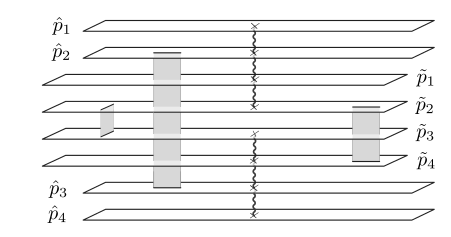
\includegraphics[width=0.75\textwidth]{../graphics/cuts}
	\caption{Examples of cuts connecting the eight sheets of the Riemann surface corresponding to the spectral curve for strings in $AdS_5 \times S^5$. The wavy line corresponds to the pole at $x = 1$.}
	\label{fig:cuts}
\end{figure}

Since the Lax connection has poles at $x = \pm 1$, so do the quasi-momenta. Due to the Virasoro constraint, which comes about from the diffeomorphism invariance of the worldsheet, the residues of the quasi-momenta are constrained to
\begin{equation}
	\{ \hat{p}_1, \; \hat{p}_2, \; \hat{p}_3, \; \hat{p}_4 \; | \; \tilde{p}_1, \; \tilde{p}_2, \; \tilde{p}_3, \; \tilde{p}_4 \} = \frac{\{ \, \alpha_{\pm}, \, \alpha_{\pm}, \, \beta_{\pm}, \, \beta_{\pm}, \, | \, \alpha_{\pm}, \, \alpha_{\pm}, \, \beta_{\pm}, \, \beta_{\pm} \}}{x \pm 1}.
\end{equation}
An additional constraint on the quasi-momenta comes from the fact that the algebra $\mathfrak{psu(2,2|4)}$ has an automorphism, which is the cause for an additional $\mathbb{Z}_4$ grading. The constraints are given by \cite{sakura}
\begin{eqnarray}
	\tilde{p}_{1,2}(x) & = & -\tilde{p}_{2,1}(1/x) - 2 \pi m \nonumber \\
	\tilde{p}_{3,4}(x) & = & -\tilde{p}_{4,3}(1/x) - 2 \pi m \nonumber \\
	\hat{p}_{1,2,3,4}(x) & = & -\hat{p}_{2,1,4,3}(1/x).
\end{eqnarray}
These relations define an inversion symmetry. Finally one can look at the asymptotics of the quasi-momenta as the spectral parameter becomes infinite. In this limit the Lax connection becomes related to the Noether currents of the theory and hence one can relate the quasi-momenta to the charges of the global symmetry algebra by \cite{algebraic_curve}
\begin{equation}
\left(
\begin{array}{c}
  \hat{p}_1 \\
  \hat{p}_2 \\
  \hat{p}_3 \\
  \hat{p}_4 \\
  \hline
  \tilde{p}_1 \\
  \tilde{p}_2 \\
  \tilde{p}_3 \\
  \tilde{p}_4 \\
\end{array}
\right) = \frac{2 \pi}{x}
\left(
\begin{array}{c}
  + \mathcal{E} - \mathcal{S}_1 + \mathcal{S}_2 \\
  + \mathcal{E} + \mathcal{S}_1 - \mathcal{S}_2 \\
  - \mathcal{E} - \mathcal{S}_1 - \mathcal{S}_2 \\
  - \mathcal{E} + \mathcal{S}_1 + \mathcal{S}_2 \\
  \hline
  + \mathcal{J}_1 + \mathcal{J}_2 - \mathcal{J}_3 \\
  + \mathcal{J}_1 - \mathcal{J}_2 + \mathcal{J}_3 \\
  - \mathcal{J}_1 + \mathcal{J}_2 + \mathcal{J}_3 \\
  - \mathcal{J}_1 - \mathcal{J}_2 - \mathcal{J}_3 \\
\end{array}
\right),
\label{eq:asymptotics}
\end{equation}
where the charges are rescaled by $\mathcal{Q} = Q / \sqrt{\lambda}$. Thus we see that we can characterize the quasi-momenta by describing their behaviour at poles and under symmetries, by their asymptotics and their filling fractions. 

Let us now revisit the simplest string solution we know, the BMN string and describe it using the spectral curve. Not surprisingly it is the simplest algebraic curve possible, containing no poles or cuts except the trivial ones at $x = \pm 1$. The quasi-momenta are given by \cite{bmn_from_curve}
\begin{equation}
	\tilde{p}_{1,2} = -\tilde{p}_{3,4} = \hat{p}_{1,2} = -\hat{p}_{3,4} = \frac{2 \pi \mathcal{J} x}{x^2 - 1}.
\end{equation}
From the asymptotic behaviour as $x \rightarrow \infty$ we can determine the charges of this solution by comparing to (\ref{eq:asymptotics}) and we find
\begin{equation}
	\mathcal{J}_1 = \mathcal{J}, \;\;\;\;\; \mathcal{E} = \kappa = \mathcal{J},
\end{equation}
all other charges being zero. Many other solutions can be characterized this way, e.g. the giant magnon corresponds to a two cut solution \cite{gromov_quasiclassical}.

As already mentioned, the key advantage of describing solutions using algebraic curves is the ability to solve the spectral problem without actually solving the equations of motion. We already saw this at the classical level, where finding the energy of a solution amounts to looking at the asymptotic behaviour of the quasi-momenta. Quasi-classical analysis of the spectral curve enables one to go beyond the classical theory and find quantum corrections to the energy levels of classical solutions. The idea of quasi-classical analysis and the spectral curve for that matter traces back to the early days of quantum mechanics. Consider a particle in a smooth one dimensional potential described by the wave function $\psi(x)$. Define the quasi-momentum by
\begin{equation}
	p(x) \equiv \frac{\hbar}{i} \frac{\psi'(x)}{\psi(x)},
\end{equation}
the Schr\"{o}dinger equation then looks like
\begin{equation}
	p^2(x) - i \hbar \, p'(x) = 2m (E - V),
\end{equation}
which would be the classic energy momentum relation if it were not for the $\hbar$ term. The quasi-momentum has a pole for each zero of the wave function, so for a highly excited state this will be some big number $N \rightarrow \infty$ and we would recover the classical solution. What is more, the poles get closer and closer to each other and in the classical limit they condense to form a cut connecting two sheets in a Riemann surface. Thus in the classical limit we recover the spectral curve of this system. We also know that the number of poles is given by
\begin{equation}
	\frac{1}{2 \pi \hbar} \oint_\mathcal{C} p(x) \, dx = N,
\end{equation}
which is also the Bohr-Sommerfield quantization condition. This integral effectively measures the size of the cut when the poles condense to a cut, thus this is the filling fraction. This simplified discussion illustrates how one could go from a classical system to a quantum one. The idea of quasi-classical analysis is to start with a classical solution and perturb it by adding microscopic cuts to the Riemann surface, which effectively describe some quantum excitations. This is exactly what has been done for various string solutions in $AdS_5 \times S^5$ \cite{gromov_quasiclassical}. One can then proceed with comparing the spectra of string solutions beyond the classical level with spectra of spin chain states at higher loop levels and the results so far have been encouraging \cite{gromov_psu}.



Describe flat connections, monodromies, sheets etc.

\subsubsection{Folded string}

Give solution.

\subsection{String quantization and semi-classics}

Describe the quantization procedure. Derive next coefficient for Konishi.

\subsection{Short strings}



%\section{Folded string}
The folded string is the strong coupling counterpart of the Wilson operators $\tr(D^S Z^J)$.
This class of operators in particular contains the Konishi operator that has been receiving a lot of attention recently.
%\subsection{Tree level}
The classical energy of the folded string is a function of the Lorentz spin $S$,
twist $J$ and the mode number $n$. This function can be written in a parametric form
in terms of the branch points $a$ and $b$ \cite{Gromov:2011de,Beisert:2003ea,Kazakov:2004qf,Kazakov:2004nh}:
\beqa
\nn{2\pi {\cal S}}&=&\frac{ab+1}{ab}\[b E\(1-\tfrac{a^2}{b^2}\)-aK\(1-\frac{a^2}{b^2}\)\]\;,\\
{2\pi {\cal J}}&=&\frac{2\sqrt{(a^2-1)(b^2-1)}}{b}K\(1-\frac{a^2}{b^2}\)\;,\\
\nn{2\pi {\cal D}_{\rm tree}}&=&\frac{ab-1}{ab}\[b E\(1-\tfrac{a^2}{b^2}\)+aK\(1-\frac{a^2}{b^2}\)\]\;.
\eeqa
where ${\cal S},{\cal J},{\cal D}=\frac{S}{n\sqrt\lambda},\frac{J}{n\sqrt\lambda},\frac{\Delta}{n\sqrt\lambda}$.
In this paper we will concentrate on a special limit when $S$ is sent to zero.
In this limit one can write a more explicit expression for the square of the scaling dimension:
%\beqa
% {\cal D}_{\rm tree}&=&{\cal J}
%+\frac{\sqrt{{\cal J}^2+1} }{{\cal J}}{\cal S}
%-\frac{{\cal J}^2+2}{4 \left({\cal J}^5+{\cal J}^3\right)}{\cal S}^2
%+\frac{3 {\cal J}^6+13 {\cal J}^4+20 {\cal J}^2+8}{16 {\cal J}^5 \left({\cal J}^2+1\right)^{5/2}}{\cal S}^3\\
%&-&\frac{21 {\cal J}^{10}+138 {\cal J}^8+385 {\cal J}^6+540 {\cal J}^4+336
%   {\cal J}^2+80 }{128 {\cal J}^7 \left({\cal J}^2+1\right)^4}{\cal S}^4
%\nn+{\cal O}({\cal S}^5)
%\eeqa
\beqa
 {\cal D}_{\rm tree}^2&=&{\cal J}^2+2 \, {\cal S} \, \sqrt{{\cal J}^2+1}+{\cal S}^2 \, \frac{2 {\cal J}^2+3}{2
   {\cal J}^2+2}-{\cal S}^3 \, \frac{{\cal J}^2+3}{8
   \left({\cal J}^2+1\right)^{5/2}}
   %+{\cal S}^4\frac{3 {\cal J}^4+18 {\cal J}^2+31}{64 \left({\cal J}^2+1\right)^4}
   +{\cal O}\left({\cal S}^4\right)\;.
\eeqa
One can easily see that the coefficients in the expansion of ${\cal D}_{\rm tree}^2$
are considerably simpler than the same coefficients in the expansion of ${\cal D}_{\rm tree}$.

One can further notice \cite{Basso:2011rs} that the re-expansion of the function $\Delta^2$ in the large $\mu\equiv \lambda n^2$ limit with $S$ and $J$ fixed has a particularly nice structure
\beq
\Delta_{\rm tree}^2\!\!\!=\!J^2+S
\(
2\, \sqrt{\mu}+\frac{J^2}{\sqrt{\mu}}+\dots%-\frac{J^4}{4\mu^{3/2}}
\)
+S^2
\(
\frac{3}{2}-\frac{J^2}{2\mu}
+\dots%+\frac{J^4}{2\mu^2}
\)
-S^3
\(
\frac{3}{8\sqrt{\mu}}
-\frac{13 J^2}{16\sqrt[3]{\mu}}
+\dots
\)
%+S^4\(\frac{31}{64\mu}+\dots\)
+{\cal O}({ S}^4)
\label{dsquare_tree}
\eeq
where each next term in $S$
gets more and more suppressed for large $\lambda$.
This structure indicates that the expansion in large $\lambda$
and small $S$ should be easily computable, which is very important in the study of short operators. 
The structure in \eq{dsquare_tree} is a purely classical result. In the next section we discuss whether it is preserved when quantum corrections are taken into account.


%\subsection{One loop}
Using the algebraic curve technique \cite{Gromov:2009zza,Gromov:2007aq,Gromov:2007ky,Gromov:2008ec,SchaferNameki:2010jy}
the result \eq{dsquare_tree} at one loop can be shown to be just a little bit more involved than the classical energy.
The derivation is described in \cite{Gromov:2011de} so we only quote the result here (see appendix \ref{appA} for more details).

Again, in the limit when ${\cal S}$ is sent to zero the result simplifies significantly.
Up to two orders in $\mathcal{S}$ we found the following expansion
\beqa
\label{delta_oneloop}
\Delta_{\rm 1-loop}&\simeq&
\frac{-{\cal S}}{2 \left({\cal J}^3+{\cal J}\right)}+{\cal S}^2\[\frac{3 {\cal J}^4+11 {\cal J}^2+17
   }{16 {\cal J}^3 \left({\cal J}^2+1\right)^{5/2}}
%   -\frac{\left(6 {\cal J}^8+48 {\cal J}^6
%   +138
%   {\cal J}^4+
%   352 {\cal J}^2+117\right) {\cal S}^3}{64 {\cal J}^5 \left({\cal J}^2+1\right)^4}
\!-\!\sum_{m>0,m\neq n}\frac{n^3m^2  \left(2 m^2+n^2 {\cal J}^2-n^2\right)}{{\cal J}^3 \left(m^2-n^2\right)^2
   \left(m^2+n^2 {\cal J}^2\right)^{3/2}}\]
   \;.
\eeqa
The next term in this expansion can be found in \eq{delta_oneloop_3}, \eq{delta_oneloop_4}. The sum is nothing but a sum over the fluctuation energies,
whereas the remaining terms originate from the ``zero"-modes
$m=n$, which have to be treated separately.
The sum can be very easily expanded for small ${\cal J}$.
It is easy to see that the expansion coefficients will be certain combinations
of zeta-functions. It is also easy to see that
the dependence on the mode number $n$ is rather nontrivial.

The expansion of the one loop energy first in small ${\cal S}$
up to a second order and then in small ${\cal J}$ reads
%\beq
%\Delta_{\rm1-loop}=
%-\frac{{\cal S}}{2 {\cal J}^3+2{\cal J}}
%+{\cal S}^2\(
%\frac{1}{2{\cal J}^3}-
%\frac{3\zeta_3-\frac{1}{8}}{2\cal J}+\dots
%\)+{\cal O}({\cal S}^3)\;.
%\eeq
\beq
\label{delta_oneloop_sj}
\Delta_{\rm1-loop}\simeq
\left\{
\begin{array}{ll}
 -\frac{\mathcal{S}}{2 \mathcal{J}}+
 \mathcal{S}^2 \left(+\frac{1}{2\mathcal{J}^3}-\frac{3 \zeta_3}{2 \mathcal{J}}-\frac{1}{16 \mathcal{J}}\right) & \;\;,\;\;n=1 \\
 -\frac{\mathcal{S}}{2 \mathcal{J}}+
 \mathcal{S}^2 \left(+\frac{1}{2
   \mathcal{J}^3}-\frac{12 \zeta_3}{\mathcal{J}}-\frac{17}{16 \mathcal{J}}\right) & \;\;,\;\;n=2 \\
 -\frac{\mathcal{S}}{2 \mathcal{J}}+
 \mathcal{S}^2 \left(-\frac{5}{8
   \mathcal{J}^3}-\frac{81 \zeta_3}{2 \mathcal{J}}-\frac{7}{4 \mathcal{J}}\right) & \;\;,\;\;n=3 %\\
% -\frac{\mathcal{S}}{2 \mathcal{J}}+
% \mathcal{S}^2 \left(-\frac{55}{18
%   \mathcal{J}^3}-\frac{96 \zeta_3}{\mathcal{J}}-\frac{281}{144 \mathcal{J}}\right) & \;\;,\;\;n=4
\end{array}
\right.
\eeq
Expansions up to four orders in $\mathcal{S}$ and then in $\mathcal{J}$ are given in appendix \ref{AppS4}. We note that the contributions ${\cal S}^2/{\cal J}^3$
are universal for $n=1$ and $n=2$,
however starting from $n=3$ we get some nasty coefficient.
As we will discuss in the next section this could imply that
the naive generalization of the conjecture in \cite{Basso:2011rs} is not fully correct
for $n>2$. Also for $n=2$ we found  a similar anomaly at the order $S^3$.
%\section{Discussion of the exact slope and its generalizations}
Let us take a close look at the conjecture in \cite{Basso:2011rs}. It says that
making expansions of the scaling dimension squared first in ${\cal S}\to 0$
and then in $\mu\to \infty$ should reveal the following structure
\beq\label{Delta}
\Delta^2=J^2+S
\(
A_1\sqrt{\mu}+A_2+\dots
\)
+S^2
\(
B_1+\frac{B_2}{\sqrt\mu}
+\dots%+\frac{J^4}{2\mu^2}
\)
%+S^3
%\(
%\frac{C_1}{\mu^{1/2}}
%+\frac{C_2}{\mu^{3/2}}
%+\dots
%\)
%+S^4\(\frac{31}{64\mu}+\dots\)
+{\cal O}({ S}^3)\;,
\eeq
where the coefficients $A_i,\;B_i,\;C_i$ are some functions of $J$.
This is, as can be easily seen, a nontrivial constraint on $\Delta$ itself as
\beqa\label{cons}
\Delta&=&J+\frac{S}{2J}
\(
A_1\sqrt{\mu}+A_2+\frac{A_3}{\sqrt{\mu}}+\dots
\)\\
\nn&+&S^2
\(
- \frac{A_1^2}{8J^3} \, \mu
-  \frac{A_1A_2}{4J^3} \, \sqrt{\mu}
+\[\frac{B_1}{2J}-\frac{A_2^2+2A_1 A_3}{8J^3}\]
+
\[
\frac{B_2}{2J}
-\frac{A_2A_3+A_1A_4}{4J^3}
\]  \frac{1}{\sqrt\mu}
+\dots
\)
+{\cal O}(S^3)\;.
\eeqa
One of the results of \cite{Basso:2011rs}
is the exact formula for all the coefficients $A_i$. They can be found easily by expanding
a simple combination of Bessel functions, called the ``slope", around infinity and it produces~\cite{Basso:2011rs}:
\beq
A_1=2\;\;,\;\;
A_2=-1\;\;,\;\;
A_3=J^2-\frac{1}{4}\;\;,\;\;
A_4=J^2-\frac{1}{4}\dots\;.
\label{As}
\eeq
Comparing with our one-loop result we get\footnote{$B_2=-b$ in the notations of \cite{Basso:2011rs}.
The $-3\zeta_3$ term also arises in the formalism of \cite{Vallilo:2011fj} when formally extended to two loops.
A very similar $\zeta_3$ term can be also extracted from \cite{Roiban:2011fe}.
This gives extra support to our results.
We would like to thank L.Mazzucato and A.Tseytlin for pointing this out.
}
\beq\label{BB}
B_1=\frac{3}{2}\;\;,\;\;
B_2=
\left\{
\bea{ll}
-3\,\zeta_3+\frac{3}{8}&\;\;,\;\;n=1\\
-24\,\zeta_3-\frac{13}{8}&\;\;,\;\;n=2\\
-81\,\zeta_3-\frac{24}{8}&\;\;,\;\;n=3
\eea
\right.\;.
\eeq
We should, however, notice that for $n>1$ we were not able to fully satisfy \eq{cons}.
One example is the coefficient in front of $S^2/J^3$, which for $n=3$ is $-5/8$, whereas \eq{cons} predicts $1/2$. We observe that only for $S^2$, $S^3$ and higher order terms do we find such disagreements and it is interesting to note that the coefficients for $S$ order terms seem to be correct for any $n$\footnote{We indeed verified numerically that the naive replacement $\lambda\to n^2\lambda$ works at weak coupling at least to two loops.}.
These observations imply that the generalization of the original slope function,
which is done by a naive replacement $\lambda\to n^2\lambda$, is not correct for the cases when $n>1$ and thus either the coefficients in \eq{As} or the conjecture itself should be modified to accommodate this.
We discuss this in details in the next section \ref{inconsistencies}.

%\subsection{Inconsistencies in the next orders}\label{inconsistencies}

The analysis in the previous sections was done only up to second order in the small $S$ expansion. The appendix \ref{AppS4} contains our result for the
one-loop quantization of the $n$-times folded string up to the order $S^4$. For $n=1$ our result is in perfect agreement with the conjectured structure \eq{Delta}, yet for cases with $n>1$ there are inconsistencies.
For $n=2$ the first inconsistency appears in the $\frac{S^3\mu}{J^4}$ term and for $n=3$ there are already inconsistencies at order $S^2$. We found that for $n>1$ one has to modify the structure in \eq{Delta} by
including negative coefficients in order for it to be consistent with our one-loop results. E.g. for $n=2$ the structure has to be modified starting with the $S^3$ term, which now becomes
\beq
\(
C_{-2}\;\mu+\frac{C_1}{\sqrt\mu}+\frac{C_2}{\mu}+\dots
\) S^3
\eeq
with $C_{-2}=\frac{12}{J^4}$. To the next order in $S$ we find
\beq
\(
D_{-4}\;\mu^{3/2} +D_{-2}\;\sqrt{\mu}+ \frac{D_{0}}{\sqrt\mu}+\frac{D_1}{\mu}+\dots
\) S^4
\eeq
where $D_{-4}=-\frac{78}{J^6},\;D_{-2}=-\frac{36}{J^4},\;D_0=\frac{21}{2J^2}$.

For $n=3$ the first modification already occurs at order $S^2$ and it can be resolved if the term $-\frac{9 S^2\sqrt\mu}{4 J^2}$ is added to \eq{Delta}.
Thus effectively the conjectured structure \eq{Delta} has to be modified as in the $n=2$ case by including negative coefficients, which now depend on $n$ in a nontrivial way.
It is also worth noticing that since inconsistencies start appearing at orders of $\frac{S^2}{J^2}$ and $\frac{S^3}{J^4}$ for $n=3$ and $n=2$ respectively, one might guess that
there should be an inconsistency at order $\frac{S^4}{J^6}$ for $n=1$, however we found no such thing.

This study of inconsistencies reveals that the proposed modifications to the structure of \eq{Delta} have growing powers of $\mu$,
thus one should resum them together with similar singular terms which may arise in higher loop levels before being able to make justified predictions
for short operators ($S\sim J\sim 1$) at strong coupling when $n>1$.


%\section{Two loop prediction}
The equation \eq{Delta} allows one to
make a very nontrivial prediction for the strong coupling
expansion of operators with fixed length $J$ and
the number of derivatives $S$. For that end we simply fix $S$ and $J$ in \eq{Delta}
and expand for large $\lambda$ or, equivalently, $\mu$. This procedure gives:
\beq
\Delta_{S,J,n}\simeq\sqrt{2S}\mu^{1/4}
+\frac{2J^2+3S^2-2S}{4\,(2 S)^{1/2}\,\mu^{1/4}}
+\frac{-21S^4+(32B_2+12)S^3+(20J^2-12)S^2+8J^2 S-4J^4}{32\,(2S)^{3/2}\,\mu^{3/4}}\;
\eeq
where $B_2$ is given in \eq{BB}.
Note that according to our observations there are some inconsistencies in the conjecture that this derivation relies on when $n>1$ and thus this result should be treated with great care.\footnote{We assume that the results of \cite{Basso:2011rs} for the slope function
can be lifted by generalizing with the simple replacement $\lambda\to n^2\lambda$ when $n>1$. 
We indeed verified this numerically with high precision at weak coupling up to two loops and this is also in agreement
with our one loop strong coupling results. I.e. the slope function and hence the coefficients $A_i$ in \eq{As} are still correct after the replacement, but as argued before, the structure of the expansion \eq{Delta} may need to be modified.}
%These cases, however, were not analyzed as thoroughly
%as the $n=1$ case in \cite{Basso:2011rs} where some additional tests at weak coupling were made.

Let us write the result more explicitly for a particular important case of two magnons
\beq
\Delta_{2,J,1}=2 \, \lambda^{1/4}+
\frac{\frac{J^2}{4}+1}{\lambda^{1/4}}+\frac{-\frac{J^4}{64}+\frac{3 J^2}{8}-3\, \zeta
   (3)-\frac{3}{4}}{\lambda^{3/4}}\;.
\eeq
In the next section we compare our prediction with the available TBA data.


In order to extract strong coupling asymptotics from available TBA data, we performed numerical fits of Pad\'{e} type. First we changed variables from $\lambda$ to 
\begin{equation}
	y(\lambda) = \sqrt{\lambda} \frac{\partial}{\partial\sqrt{\lambda}} \log I_2(\sqrt{\lambda}) - 2,
\end{equation}
which seems arbitrary, but nevertheless is convenient because scaling dimension dependence on $y$ looks nearly linear and automatically captures some important analytical features. We then represent the scaling dimension as the square root of a rational function of two polynomials in $y$ with some of the unknown coefficients chosen so as to fix the leading order weak and strong coupling behaviours. So for example, for the Konishi operator we chose
\begin{equation*}
	\Delta_{2,2,1} = \sqrt{18 + 4y + \frac{-2 + \sum_{i=1}^{P} a_i y^i}{1 + \sum_{i=1}^{P+1} b_i y^i}},
\end{equation*}
because one can easily verify that the weak coupling expansion of this function is given by
\begin{equation*}
	\Delta_{2,2,1} = 4 + \mathcal{O}(g^2),
\end{equation*}
and the strong coupling expansion is given by
\begin{equation*}
	\Delta_{2,2,1} = 2 \lambda^{1/4} + \frac{2}{\lambda^{1/4}} + \mathcal{O}(\lambda^{-3/4}).
\end{equation*}
This way the leading order behaviour is fixed and next to leading order coefficients are combinations of the unknowns $a_i$ and $b_i$, which we then find by the method of least squares. The number of fit coefficients $P$ is chosen so that their values after fitting would be of order one, which would imply that the fit is reasonable. Though the procedure seems ad hoc, it produces incredibly good fits, which agree very well with both weak and strong coupling expansions. Fits to available TBA numerical data are shown in Fig. \ref{fig:frolov_compare}, where dots represent numerical values and the solid lines are our fits\footnote{For some of the fits we took the first 50 points from the corresponding data set, since we suspected the precission to be lower for higher values of $\lambda$. Also, these points were enough to get stable fits.}. Expanding our fits in powers of $\lambda$ at strong coupling we were able to compare the $\lambda^{-3/4}$ coefficients in the expansions to our predictions. These are summarized in Table \ref{tab:coefficients} for various operators. We see that our predictions agree with numerical data very well. The table also lists the weak coupling expansion coefficients of $g^2$ (tree level is fixed by hand), which agree with remarkable precision to Bethe ansatz predictions, once again indicating that the fits work well in both ends of the coupling range.

\begin{table}[t]
\begin{tabular}{|l||rl|l|l||l|l|l|}
  \hline
  $(S,J,n)$ & \multicolumn{2}{|l|}{$(n^2 \lambda)^{-3/4}$ prediction} & $(n^2 \lambda)^{-3/4}$ fit & error & $g^2$ analytical & $g^2$ fit & fit order\\
  \hline
  $(2,2,1)$ & $1/2 - \zeta_3 $&$= -3.1062$ & $-3.0739$ & $1.0\%$ & $12$ & $12.0108$ & 6\\
  $(2,3,1)$ & $87/64 - 3\,\zeta_3 $&$= -2.2468$ & $-2.2296$ & $0.8\%$ & $8$ & $8.0039$ & 5 \\
  $(2,4,2)$ & $-3/4 -24 \, \zeta_3 $&$= -29.5994$ & $-30.0547$ & $1.5\%$ & $14.4721$ & $14.4428$ & 5\\
  \hline
\end{tabular}
\caption{Comparisons of strong coupling expansion coefficients for $\lambda^{-3/4}$ obtained from fits to TBA data versus our predictions for various operators. The weak coupling expansion coefficients for $g^2$ show how well the fit approximates the data. The fit order is the order of polynomials used for the rational fit function.}
\label{tab:coefficients}
\end{table}

We also tried comparing our predictions to numerical data for the operator $S=2,J=4,n=2$ (see Fig. \ref{fig:frolov_compare} and Table \ref{tab:coefficients}). As argued before, since this operator has $n>1$, we cannot fully trust our result in this case, nevertheless the result agrees well with the numerical fits we get and the error is only slightly bigger than for the $n=1$ states. It is hard to draw conclusions about this, as there is not a lot of numerical data available for such operators. 




% This section describes the work performed by the author which culminated in the publication \cite{Gromov:2011bz}, which itself is largely based on the semiclassical analysis performed in \cite{Gromov:2011de}. 

% Here we are interested in the so called $SL(2)$ sector of the theory, which is composed of operators of the form $\mathrm{Tr}( D^S Z^J ) + \mathrm{permutations}$, where $D$ is the covariant derivative, $S$ is the spin and $J$ is the angular momentum of the operator. This sector is convenient, since equations suitable for numerical studies were formulated for it and thus one can cross check everything against numerics. On the string theory side operators from this sector correspond to the so-called spinning folded strings. At the classical level, it is convenient to describe them in terms of the scaled charges $\mc S = S/\sqrt\lambda$, $\mc J = J/\sqrt\lambda$. They have a simple and clear dynamical meaning: the spin $\mc S$ is associated with rotation around the center of  $AdS_{5}$ while $\mc J$ is an angular momentum on the sphere. At small $\mc S$, the string is short and admits a near-flat space description. At large $\mc S$, the string stretches and reaches the boundary of $AdS$ with the characteristic scaling $E \sim \log \mc S$ of its energy. Short strings are especially interesting, since their strong coupling limit looks very difficult to address both within the gauge theory and perturbative string theory approaches, on the other hand, quantum corrections in the semiclassical approximation are fully under control and can be studied by algebraic curve tools.

% The algebraic curve method is one of the most advanced ways of computing the semi-classical corrections AdS/CFT. The method is heavily based on integrability and is naturally free from any perturbation theory ambiguities. The only input needed to proceed with the quantization is a set of quasi-momenta $\hat p_i,\, \tilde p_i,\;i=1,2,3,4$ which were mentioned in the previous section on integrability. In particular, the folded string solution corresponds to the curve with two symmetric cuts with real branch-points $\pm b, \pm a$ such that $1<a<b$. The explicit form of the quasi-momenta depends on the twist $J$ and the Lorentz spin $S$ and can be constructed using the methods of \cite{Beisert:2003ea}, \cite{Kazakov:2004qf}, \cite{Kazakov:2004nh}. 
  
% A more detailed description of the procedure will be given in the following section on $AdS_4/CFT_3$, since the author has performed the analysis in that case and published the result in \cite{Beccaria:2012qd} \cite{Beccaria:2012vb}. At this stage the take away point is that the semiclassical quantization procedure produces the following result for the energy of a folded string up to one loop level
 % \beq \Delta^{\rm classical}+\delta E=\lambda^{1/4}\sqrt{2S}
 % +\frac{1}{\lambda^{1/4}}\frac{2J^2+S(3S-2)}{4\sqrt{2S}}\;.  \eeq

% The authors contribution to the $AdS_5/CFT_4$ case is the publication \cite{Gromov:2011bz}, which builds on top of the aforementioned semiclassical analysis in the following way. Consider the limit $\cal{S} \rightarrow \mathrm{0}$ where the semiclassical correction to the string energy can be written as
% \beqa
% \label{delta_oneloop}
% \delta E &\simeq&
% \frac{-{\cal S}}{2 \left({\cal J}^3+{\cal J}\right)}+{\cal S}^2\[\frac{3 {\cal J}^4+11 {\cal J}^2+17
   % }{16 {\cal J}^3 \left({\cal J}^2+1\right)^{5/2}}
% \!-\!\sum_{m>0,m\neq n}\frac{n^3m^2  \left(2 m^2+n^2 {\cal J}^2-n^2\right)}{{\cal J}^3 \left(m^2-n^2\right)^2
   % \left(m^2+n^2 {\cal J}^2\right)^{3/2}}\]\;.
% \eeqa
% If the parameters $\cal{S}$ and $\cal{J}$ are fixed to some values then the sums can be evaluated. Note that this expression mixes various orders of the coupling. Now consider the conjecture in \cite{Basso:2011rs}. It says that making expansions of the scaling dimension squared first in ${\cal S}\to 0$ and then in $\lambda\to \infty$ should reveal the following structure
% \beq
% \Delta^2=J^2+S
% \(
% A_1\sqrt{\mu}+A_2+\dots
% \)
% +S^2
% \(
% B_1+\frac{B_2}{\sqrt\mu}
% +\dots%+\frac{J^4}{2\mu^2}
% \)
% +{\cal O}({ S}^3)\;,
% \eeq
% where the coefficients $A_i,\;B_i,\;C_i$ are some functions of $J$ and $\sqrt{\mu} = n \sqrt{\lambda}$ with $n$ being the mode number. This is, as can be easily seen, a nontrivial constraint on $\Delta$ itself as
% \beqa
% \Delta&=&J+\frac{S}{2J}
% \(
% A_1\sqrt{\mu}+A_2+\frac{A_3}{\sqrt{\mu}}+\dots
% \)\\
% \nn&+&S^2
% \(
% - \frac{A_1^2}{8J^3} \, \mu
% -  \frac{A_1A_2}{4J^3} \, \sqrt{\mu}
% +\[\frac{B_1}{2J}-\frac{A_2^2+2A_1 A_3}{8J^3}\]
% +
% \[
% \frac{B_2}{2J}
% -\frac{A_2A_3+A_1A_4}{4J^3}
% \]  \frac{1}{\sqrt\mu}
% +\dots
% \)
% +{\cal O}(S^3)\;.
% \eeqa
% One of the results of \cite{Basso:2011rs} is the exact formula for all the coefficients $A_i$. They can be found easily by expanding a simple combination of Bessel functions, called the ``slope", around infinity and it produces~\cite{Basso:2011rs}:
% \beq
% A_1=2\;\;,\;\;
% A_2=-1\;\;,\;\;
% A_3=J^2-\frac{1}{4}\;\;,\;\;
% A_4=J^2-\frac{1}{4}\dots\;.
% \eeq
% Comparing with our one-loop result \ref{delta_oneloop} we can also find the $B_i$'s,
% \beq
% B_1=\frac{3}{2}\;\;,\;\;
% B_2=
% \left\{
% \bea{ll}
% -3\,\zeta_3+\frac{3}{8}&\;\;,\;\;n=1\\
% -24\,\zeta_3-\frac{13}{8}&\;\;,\;\;n=2\\
% -81\,\zeta_3-\frac{24}{8}&\;\;,\;\;n=3
% \eea
% \right.\;.
% \eeq
% The equation \ref{Delta} allows one to make a very nontrivial prediction for the strong coupling expansion of operators with fixed length $J$ and the number of derivatives $S$. For that end we simply fix $S$ and $J$ in \ref{Delta} and expand for large $\lambda$ or, equivalently, $\mu$. This procedure gives:
% \beq
% \Delta_{S,J,n}\simeq\sqrt{2S}\mu^{1/4}
% +\frac{2J^2+3S^2-2S}{4\,(2 S)^{1/2}\,\mu^{1/4}}
% +\frac{-21S^4+(32B_2+12)S^3+(20J^2-12)S^2+8J^2 S-4J^4}{32\,(2S)^{3/2}\,\mu^{3/4}}\;
% \eeq
% where $B_2$ is given in \ref{BB}. Note that according to our observations there are some inconsistencies in the conjecture that this derivation relies on when $n>1$ and thus this result should be treated with great care.

% The end result is that we were able to boost the one loop result \ref{eq:loopres} to two loops simply by utilizing Basso's conjecture. We checked the prediction against exact TBA results and the agreement was very convincing.

\subsection{Towards the full solution}

Mention nested BAE, full psu(2,2|4) spin chain without going into much detail.
